% !TeX program = pdflatex
% !TeX encoding = UTF-8
\documentclass[journal]{IEEEtran}
\usepackage{amsmath}
\usepackage{float}
\usepackage{amsfonts}
\usepackage{amssymb}
\usepackage{bm}
\usepackage{graphicx}
\usepackage{booktabs}
\usepackage{placeins}
\usepackage{xurl}
\usepackage{balance}
\usepackage{tikz}
\usetikzlibrary{arrows.meta,positioning}
\usepackage[hidelinks]{hyperref}

\hypersetup{
  pdftitle={Evaluating Spatial Discriminability Preservation in HRTF Upsampling Using Fisher Information},
  pdfauthor={Dominic Bassett},
  pdfsubject={Evaluation of spatial discriminability preservation in HRTF upsampling},
  pdfkeywords={Fisher information, HRTF, spatial audio, spatial discriminability, upsampling}
}

\setlength{\textfloatsep}{5pt plus 1pt minus 2pt}
\setlength{\floatsep}{5pt plus 1pt minus 2pt}
\setlength{\intextsep}{5pt plus 1pt minus 2pt}
\setlength{\abovecaptionskip}{3pt plus 1pt minus 1pt}
\setlength{\belowcaptionskip}{0pt}

\title{Evaluating Spatial Discriminability Preservation in HRTF Upsampling Using Fisher Information}
\author{Dominic Bassett%
\thanks{D. Bassett is an independent researcher, Birmingham, U.K. (e-mail: dominicbassett04@gmail.com). This work develops research begun for his B.Sc. dissertation at Birmingham City University.}}

\begin{document}

\maketitle

\begin{abstract}
HRTF upsampling is typically evaluated using signal-domain reconstruction metrics and statistical localisation models, but neither directly assesses whether a listener could still distinguish neighbouring source directions. We introduce an evaluation based on Fisher information over the sphere of source directions. Spatial gradients of positive spectral-gradient, interaural level-difference, and interaural time-difference features define a bivariate Fisher information tensor at every direction. This tensor gives a local discrimination ellipse and the Cram\'er--Rao bound on the covariance of any unbiased local estimate. Reference and reconstructed tensors are compared using the affine-invariant Riemannian metric (AIRM), which captures changes in the scale, anisotropy, and orientation of the ellipses. We evaluate SUpDEq-based interpolation, RANF, and FSP-AE on 41 SONICOM subjects at four sparse-grid retention levels, on a common 16-kHz cue band, alongside log-spectral distance (LSD) and a Bayesian localisation model. RANF best preserves the tensor field at 19, 5, and 3 retained directions, and is the only method without a systematic gain or loss of Fisher information. This ranking is unchanged under different spherical-harmonic orders and spectral noise weights. Across conditions, AIRM is strongly rank-associated with LSD, but within conditions it identifies consistent differences that LSD misses or reverses. Magnitude correction lowers LSD and predicted polar error while degrading the tensor field, and smoothing reconstructions lose discriminability that direction-wise errors cannot reveal. Without fitting, the reference tensors reproduce the directional pattern of measured minimum audible angles, including the ratio of oblique to horizontal acuity. Fisher information therefore provides a distinct, interpretable criterion for HRTF reconstruction.
\end{abstract}

\begin{IEEEkeywords}
Fisher information, head-related transfer functions, information geometry,
spatial audio, spatial discriminability, upsampling.
\end{IEEEkeywords}

\section{Introduction and Background}

Head-related transfer functions (HRTFs) describe the direction-dependent filtering introduced by a listener's head, torso, and pinnae. Because dense individual HRTF measurements are costly to obtain, spatial upsampling is used to reconstruct a dense directional field from a sparse set of measured directions. Upsampling methods are usually evaluated using log-spectral distance (LSD), interaural level-difference error, interaural time-difference error, and localisation-model metrics. The first three compare the reconstructed and reference HRTFs direction by direction, and the last predicts where a listener would point. Neither class of measure assesses how localisation cues vary between neighbouring directions, yet it is this local variation that determines whether two nearby sources can be told apart. The relevant object of evaluation is therefore not only the HRTF at each direction, but also the local structure of localisation cues over the sphere.

That local structure is known to depend on both source direction and displacement direction. Starch~\cite{Starch1905} combined horizontal and vertical discrimination measurements into ``auditory discrimination ellipses''. However, the ellipse axes were fixed to the horizontal and vertical planes, with thresholds in intermediate directions inferred from the ellipse rather than measured. The stimulus, a 100-Hz electric fork, also lacked the cross-band spectral structure needed for elevation discrimination. Whether the principal axes of spatial acuity coincide with azimuth and elevation was therefore assumed rather than tested.

Analyses of full localisation response distributions suggest that they generally do not. Carlile et al.~\cite{Carlile1997} modelled error distributions using either the isotropic Fisher distribution or the elliptical Kent distribution. In the pooled data, distributions at 50 of 76 target locations (66\%) were classified as Kent. Their major axes often departed from the azimuth/elevation axes and, rather than following the cones of confusion expected under orthogonal cue processing, showed co-latitude alignment at lateral and posterior locations and radial alignment near the frontal midline. Response distributions are not discrimination thresholds, but this structure indicates that the underlying cue sensitivity is anisotropic and obliquely oriented. A local description of spatial acuity must therefore allow its scale, anisotropy, and orientation all to vary with direction.

Current evaluation tools do not provide such a description. Reconstructions are commonly assessed with auditory observer models that convert an HRTF set into predicted localisation responses. The Bayesian model of Barumerli et al.~\cite{Barumerli2023}, used here to assess each reconstruction, combines HRTF-derived sensory evidence with a spatial prior, a maximum a posteriori (MAP) decision rule, and post-decision response variability. It yields predicted point estimates from which lateral, polar, and quadrant errors can be calculated. The original model was calibrated against aggregate localisation errors, and a later extension introduced likelihood-based fitting to complete response distributions~\cite{Barumerli2026}. In both formulations, however, the final response stage applies isotropic von Mises--Fisher scatter around each MAP estimate, so direction-dependent anisotropy is not represented at the response stage.

Capturing response anisotropy would still not be sufficient. Discrimination thresholds limit how precise localisation can be, and the two tend to share a similar shape, but they are not equivalent: localisation responses also reflect response noise, mapping, and bias, whereas discrimination reflects how rapidly sensory cues change between neighbouring directions. A reconstruction can therefore leave predicted pointing performance intact while altering the scale, anisotropy, or orientation of local spatial discriminability. A tensorial analysis of the gradients of the observer's sensory cues quantifies these properties directly, and so complements model-based localisation predictions.

Fisher information provides such a tensor. It quantifies how sensitive the expected auditory cues are to small changes in source direction, and has been used in auditory neuroscience to relate binaural cue statistics to neural coding and perception. For interaural time differences (ITDs), Harper and McAlpine~\cite{Harper2004} showed that neural tuning in the mammalian brainstem can be organised to maximise Fisher information over naturally occurring cue ranges. Pav\~ao et al.~\cite{Pavao2020} extended this analysis to human listeners, reporting that the spatial distribution of Fisher information derived from HRTF statistics correlates with measured free-field ITD discrimination thresholds. This paper applies the same quantity to the evaluation of HRTF spatial upsampling, comparing Fisher information tensors derived from reference and reconstructed auditory cue fields.

Let the sound-source direction be \(\mathbf{r}\in\mathbb{S}^2\), and let \(\boldsymbol{\xi}\in\mathbb{R}^{2}\) denote local angular coordinates in an orthonormal tangent basis at \(\mathbf{r}\). The observer is defined by a cue vector \(\mathbf q\) comprising positive spectral-gradient, interaural level-difference (ILD), and transformed ITD features, following the sensory evidence used by Barumerli et al.~\cite{Barumerli2023}. The cues are modelled as
\(\mathbf q\mid\boldsymbol{\xi}\sim
\mathcal N(\boldsymbol\mu(\boldsymbol\xi),\boldsymbol\Sigma)\),
with direction-independent internal-noise covariance \(\boldsymbol\Sigma\). \(\boldsymbol\Sigma\) is taken to be diagonal, so noise is independent across features, and in particular across monaural spectral, ILD, and ITD cues.

Consider two nearby directions separated by \(\delta\boldsymbol\xi\). Equal-covariance Gaussian signal detection theory gives
\(d'^2=\Delta\boldsymbol\mu^T\boldsymbol\Sigma^{-1}
\Delta\boldsymbol\mu\). Linearising the cue mean as
\(\Delta\boldsymbol\mu\approx\mathbf J\delta\boldsymbol\xi\), where \(\mathbf J=\partial\boldsymbol\mu/\partial\boldsymbol\xi\) is the tangent Jacobian of the cue field, yields
\begin{equation}
d'^2 \approx \delta\boldsymbol{\xi}^T
\underbrace{\mathbf J^T\boldsymbol\Sigma^{-1}\mathbf J}_{\mathbf g(\mathbf r)}
\delta\boldsymbol{\xi}.
\end{equation}
For a Gaussian observation with fixed covariance, \(\mathbf g(\mathbf r)\in\mathbb{R}^{2\times2}\) is exactly the Fisher information matrix (FIM) of \(\mathbf q\) with respect to \(\boldsymbol\xi\). Where it is positive definite, it defines a Riemannian metric on the sphere of source directions~\cite{Rao1945}, with squared infinitesimal distance
\begin{equation}
ds^2 = d\boldsymbol{\xi}^T \mathbf{g}(\mathbf{r})\, d\boldsymbol{\xi}.
\end{equation}
Distance in this metric is therefore measured in units of discriminability: a short path of length \(ds\) corresponds to a local sensitivity \(d'\approx ds\).

Writing \(\delta\boldsymbol{\xi}=\rho\mathbf{u}\), where \(\mathbf{u}\in\mathbb{R}^{2}\) is a unit tangent direction, gives the angular displacement predicted to reach \(d'=1\):
\begin{equation}
\rho_{d'=1}(\mathbf{r},\mathbf{u})
=
\left(
\mathbf{u}^T \mathbf{g}(\mathbf{r}) \mathbf{u}
\right)^{-1/2}.
\label{eq:threshold}
\end{equation}
This is the scalar threshold reported later for selected horizontal, vertical, and oblique displacements. Over all \(\mathbf u\), these thresholds trace the ellipse \(\delta\boldsymbol\xi^T\mathbf g(\mathbf r)\,\delta\boldsymbol\xi=1\), whose principal axes lie along the eigenvectors of \(\mathbf g(\mathbf r)\) with semi-axis lengths equal to the inverse square roots of its eigenvalues. The same tensor also constrains localisation. For any unbiased local estimator \(\hat{\boldsymbol{\xi}}\), provided \(\mathbf g(\mathbf r)\) is nonsingular, the Cram\'er--Rao bound (CRB) states~\cite{Dayan2001}
\begin{equation}
\operatorname{Cov}(\hat{\boldsymbol{\xi}}) \succeq \mathbf{g}(\mathbf{r})^{-1}.
\end{equation}
The one-standard-deviation ellipse of the bounding covariance \(\mathbf g(\mathbf r)^{-1}\) is the same \(d'=1\) ellipse. Within this observer, the tensor therefore determines discrimination directly but only limits localisation precision, since real responses add response noise and bias and need not be unbiased. This formalises the distinction drawn above.

Diagonal feature noise does not make the spatial tensor diagonal. For diagonal \(\boldsymbol\Sigma\), the off-diagonal entry is
\(g_{12}=\sum_i \sigma_i^{-2}(\partial_1\mu_i)(\partial_2\mu_i)\),
which is generally nonzero because cue gradients need not align with the tangent axes. Setting \(g_{12}=0\) would force the discrimination ellipses to remain axis-aligned, which is precisely the assumption that Starch's ellipses embodied and that Carlile et al.'s Kent distributions contradict. The analysis therefore retains the full tensor.

Because the tensor is built from the spatial derivatives of the cue field, it captures properties that direction-by-direction error measures do not. A reconstruction can match the reference HRTF closely at each direction while distorting how the cues change between directions, so reconstructions with similar spectral error can produce different Fisher tensors. Reference and reconstructed tensors are compared using the affine-invariant Riemannian metric (AIRM) on symmetric positive-definite matrices, which reflects differences in the size, shape, and orientation of the local discrimination ellipses. The resulting discrepancy is reported alongside signal-domain errors and Bayesian-observer simulations. Figure~\ref{fig:evaluation_pipeline} summarises the evaluation sequence.
\begin{figure}[t]
    \centering
    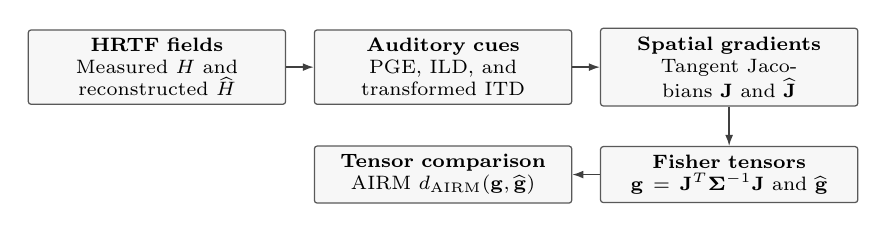
\begin{tikzpicture}[
        node distance=3.5mm,
        stage/.style={
            draw=black!65,
            fill=black!3,
            rounded corners=1pt,
            line width=0.45pt,
            align=center,
            inner xsep=2.5pt,
            inner ysep=3pt,
            font=\scriptsize,
            text width=0.255\columnwidth
        },
        flow/.style={
            -{Latex[length=1.4mm,width=1mm]},
            line width=0.5pt,
            draw=black!75
        }
    ]
        \node[stage] (hrtf) {\textbf{HRTF fields}\\Measured $H$ and reconstructed $\widehat H$};
        \node[stage, right=of hrtf] (cues) {\textbf{Auditory cues}\\PGE, ILD, and transformed ITD};
        \node[stage, right=of cues] (gradients) {\textbf{Spatial gradients}\\Tangent Jacobians $\mathbf J$ and $\widehat{\mathbf J}$};
        \node[stage, below=5mm of gradients] (tensors) {\textbf{Fisher tensors}\\$\mathbf g=\mathbf J^T\boldsymbol\Sigma^{-1}\mathbf J$ and $\widehat{\mathbf g}$};
        \node[stage, left=of tensors] (comparison) {\textbf{Tensor comparison}\\AIRM $d_{\mathrm{AIRM}}(\mathbf g,\widehat{\mathbf g})$};

        \draw[flow] (hrtf) -- (cues);
        \draw[flow] (cues) -- (gradients);
        \draw[flow] (gradients) -- (tensors);
        \draw[flow] (tensors) -- (comparison);
    \end{tikzpicture}
    \caption{Overview of the proposed evaluation. Measured and reconstructed HRTF fields are transformed into auditory cue fields, differentiated spatially, and compared through their Fisher tensors.}
    \label{fig:evaluation_pipeline}
\end{figure}

\section{Cue Feature Extraction}\label{sec:cues}
Let \(\mathbf{r}=[r_x,r_y,r_z]^T\in\mathbb{S}^{2}\) be a unit source direction. For ear \(c\in\{L,R\}\), let \(A_c(f_k,\mathbf{r})\) and \(\widehat{A}_c(f_k,\mathbf{r})\) denote the target and reconstructed HRTF magnitudes at frequency bin \(f_k\), and \(D_c\), \(\widehat D_c\) the corresponding directional transfer function (DTF) magnitudes, obtained by the same common-transfer-function (CTF) removal (SOFA \path{SOFAhrtf2dtf}, log-magnitude average) applied separately to each field. The CTF is direction-independent and carries no spatial information, so the spectral and level cues are computed from DTFs; raw HRTF magnitudes are retained for the signal-domain metrics.

The cue vector \(\mathbf q(\mathbf r)\) comprises positive spectral-gradient features for each ear, a broadband ILD, and a transformed ITD. Each is expressed on a scale on which constant internal noise is a reasonable approximation, decibels for the spectral and level cues and accumulated ITD just-noticeable differences (JNDs) for the timing cue, which justifies the direction-independent \(\boldsymbol\Sigma\) assumed above.

\subsection{Common Cue Band}
FSP-AE generates HRIRs at 32~kHz and so contains no energy above 16~kHz. To compare all methods on equal terms, every field, reference and reconstructed, is filtered before cue extraction with the same linear-phase FIR low-pass filter (order 256, Kaiser window, \(\beta=8\); flat to 15~kHz, more than 80~dB attenuation above 16~kHz), and the auditory filterbank stops at 16~kHz. The filter delay is common to both ears and all directions, so it does not alter the ITD. The same band limit is applied to the Bayesian observer (Section~\ref{sec:bayes}).

\subsection{Cue Families}
Positive spectral-gradient features (PGE) follow the sagittal-plane convention of Baumgartner et al.~\cite{Baumgartner2014}, as implemented in the Auditory Modeling Toolbox (AMT) function \path{barumerli2023_featureextraction}. DTFs are analysed by a gammatone filterbank with \(B\) centre frequencies \(f_b\) spaced at one equivalent rectangular bandwidth between 0.7 and 16~kHz. With \(m_c[b,\mathbf r]=20\log_{10}D_c(f_b,\mathbf r)\), adjacent bands are differenced and half-wave rectified,
\begin{equation}
S_c[b,\mathbf{r}]
=\max\!\left(m_c[b+1,\mathbf{r}]-m_c[b,\mathbf{r}],0\right)
\end{equation}
for \(b=1,\ldots,B-1\), and the values from both ears form the monaural spectral cue vector \(\mathbf s(\mathbf r)\in\mathbb R^{N_S}\), \(N_S=2(B-1)\). The broadband ILD is the log-ratio of the root-mean-square amplitudes of the left- and right-ear impulse responses \(x_c(t,\mathbf r)\),
\begin{equation}
\operatorname{ILD}(\mathbf{r})
= 20\log_{10}
\frac{\operatorname{rms}_t\, x_L(t,\mathbf{r})}
     {\operatorname{rms}_t\, x_R(t,\mathbf{r})},
\label{eq:ild}
\end{equation}
evaluated on the directional impulse responses for the cue field.

Because the ITD depends on interaural phase, it is estimated from the full head-related impulse responses (HRIRs) \(a_c(t,\mathbf r)\) with the broadband envelope-correlation estimator of the Barumerli feature extractor (AMT \path{itdestimator}, \path{MaxIACCe}). The same estimator gives \(\tau(\mathbf r)\) for the reference and \(\hat\tau(\mathbf r)\) for every reconstruction, including the learning-based ones, so timing errors introduced by reconstruction enter the comparison. Broadband ITD JNDs grow approximately linearly with reference ITD, \(\mathrm{JND}(\tau)\approx b+a|\tau|\), with \(a=0.095\) and \(b=32.5\,\mu\mathrm{s}\)~\cite{Reijniers2014}. Integrating the reciprocal JND gives the accumulated-JND coordinate of the observer model~\cite{Reijniers2014,Barumerli2023},
\begin{equation}
T(\tau)=\frac{\operatorname{sgn}(\tau)}{a}
\ln\!\left(1+\frac{a|\tau|}{b}\right),
\end{equation}
a variance-stabilising transformation on which constant Gaussian noise represents constant uncertainty in JND units. The ITD cue is \(\operatorname{ITD}(\mathbf{r}) = T(\tau(\mathbf{r}))\), and the full cue vector is \(\mathbf q(\mathbf r)=[\mathbf s(\mathbf r)^T,\operatorname{ILD}(\mathbf r),\operatorname{ITD}(\mathbf r)]^T\in\mathbb R^M\), \(M=N_S+2\). The same extraction applied to a reconstruction gives \(\widehat{\mathbf q}(\mathbf r)\).

\section{Continuous Spatial Gradients}
Each cue component is represented on the sphere by a truncated real spherical-harmonic (SH) basis \(\mathbf{Y}(\mathbf{r}) \in \mathbb{R}^{C}\) of maximum degree \(N_{\max}\), \(C=(N_{\max}+1)^2\). With the cues at the 793 measured directions collected in \(\mathbf{Q}\in\mathbb{R}^{793\times M}\) and the corresponding design matrix \(\mathbf{Y}_{\mathrm{fit}}\in\mathbb{R}^{793\times C}\), the least-squares coefficients are \(\mathbf{B} = \mathbf{Y}_{\mathrm{fit}}^{\dagger}\mathbf{Q}\), and the smooth field \(\widetilde{\mathbf{q}}(\mathbf{r}) = \mathbf{B}^{T}\mathbf{Y}(\mathbf{r})\) is taken as the mean cue \(\boldsymbol\mu(\mathbf r)\). The reconstructed cues are fitted in the same way, \(\widehat{\mathbf{B}} = \mathbf{Y}_{\mathrm{fit}}^{\dagger}\widehat{\mathbf{Q}}\). Both fields therefore share the same grid, basis, and degree (\(N_{\max}=6\) in the main evaluation), so differences between their gradients reflect differences between the cue fields rather than between their representations. The comparison is correspondingly restricted to spatial variation up to degree \(N_{\max}\); sensitivity to this choice is reported in Section~\ref{sec:sensitivity}.

The SH representation gives analytic derivatives at any direction. With \(\mathbf{J}_{\mathbf{Y}}(\mathbf{r})=\nabla_{\mathbf{r}}\mathbf{Y}(\mathbf{r})\in \mathbb{R}^{C\times 3}\) the Cartesian gradient of a smooth extension of the basis off the sphere, the Cartesian cue Jacobian is \(\mathbf{J}_{\mathrm{Cart}}(\mathbf{r})=\mathbf{B}^{T}\mathbf{J}_{\mathbf{Y}}(\mathbf{r})\in\mathbb{R}^{M\times3}\). Its radial component depends on the extension and has no meaning for source direction, so it is removed by projection onto the tangent plane at \(\mathbf r\). A local orthonormal basis \(\mathbf{V}(\mathbf{r})=[\mathbf{u}_1,\mathbf{u}_2]\) is constructed as
\begin{equation}
\mathbf{u}_1 = \frac{\mathbf{h}\times \mathbf{r}}{\|\mathbf{h}\times \mathbf{r}\|_2},
\qquad
\mathbf{u}_2 = \mathbf{r} \times \mathbf{u}_1,
\end{equation}
with auxiliary vector \(\mathbf{h} = [0,1,0]^T\) if \(|r_z| > 0.9\) and \([0,0,1]^T\) otherwise, avoiding a degenerate cross product near the poles. With \(x\) to the front, \(y\) to the left, and \(z\) upwards, \(\mathbf u_1\) points along increasing azimuth and \(\mathbf u_2\) along increasing elevation for \(|r_z|\le0.9\), and the tangent coordinates \(\boldsymbol\xi\) are angles in radians to first order. The tangent Jacobian \(\mathbf{J}=\mathbf{J}_{\mathrm{Cart}}\mathbf{V}\in \mathbb{R}^{M\times2}\), and likewise \(\widehat{\mathbf J}\), give the tensors \(\mathbf g=\mathbf J^T\boldsymbol\Sigma^{-1}\mathbf J\) and \(\widehat{\mathbf g}=\widehat{\mathbf J}^T\boldsymbol\Sigma^{-1}\widehat{\mathbf J}\). The same basis is used for target and reconstruction at each direction. AIRM is invariant to this choice, but individual tensor components and directional thresholds are not.

\section{Construction of the Fisher--Rao Metric Tensor}
Following the independent-feature noise model of Barumerli et al.~\cite{Barumerli2023}, \(\boldsymbol\Sigma=\operatorname{diag}(\sigma_{\mathrm{mon}}^2\mathbf I_{N_S},\sigma_{\mathrm{ILD}}^2,\sigma_{\mathrm{ITD}}^2)\), with \(\sigma_{\mathrm{mon}}=1.25\,\mathrm{dB}\), \(\sigma_{\mathrm{ILD}}=1\,\mathrm{dB}\), and \(\sigma_{\mathrm{ITD}}=0.569\) JND units on the \(T(\tau)\) scale. The ITD value is the discrimination-derived standard deviation of Reijniers et al.~\cite{Reijniers2014}. The PGE and ILD values are the medians of the listener-specific fits of Barumerli et al.~\cite{Barumerli2023}, which were calibrated against localisation responses rather than discrimination thresholds and should be read as effective observer-model weights. Two consequences follow. The absolute thresholds derived from \(\mathbf g\) are predictions of the observer model, not fits to discrimination data. And a common rescaling of all three standard deviations scales both tensors by the same factor, to which the AIRM comparison is invariant up to the small regularisation \(\eta\) defined below, so the discrepancy depends on the relative cue weights rather than the absolute noise level; sensitivity to the spectral weight is reported in Section~\ref{sec:sensitivity}.

Let \(\mathbf{j}_{u}(\mathbf{r})\in\mathbb{R}^{2}\) denote the tangent gradient of a scalar cue \(u\), that is, the corresponding row of \(\mathbf J\). Because \(\boldsymbol\Sigma\) is diagonal, the FIM is a precision-weighted sum of outer products, one per cue:
\begin{equation}
\begin{aligned}
\mathbf{g}(\mathbf{r})={}&
\frac{1}{\sigma_{\mathrm{mon}}^2}
\sum_{c\in\{L,R\}}\sum_{b=1}^{B-1}
\mathbf{j}_{S_c[b]}\mathbf{j}_{S_c[b]}^T\\
&+\frac{1}{\sigma_{\mathrm{ILD}}^2}
\mathbf{j}_{\mathrm{ILD}}\mathbf{j}_{\mathrm{ILD}}^T
+\frac{1}{\sigma_{\mathrm{ITD}}^2}
\mathbf{j}_{\mathrm{ITD}}\mathbf{j}_{\mathrm{ITD}}^T.
\end{aligned}
\label{eq:fim_sum}
\end{equation}
Each term contributes sensitivity only along its own cue gradient, so the off-diagonal entries of \(\mathbf g\) are nonzero wherever the gradients are oblique to the tangent axes. Every term is positive semidefinite, and \(\mathbf g\) is positive definite only where the cue gradients jointly span both tangent directions; elsewhere discriminability vanishes along some direction and the CRB is undefined.

Figure~\ref{fig:sonicom_kent} contrasts two observer summaries for the dense measured HRTFs. The CRB ellipses show the smallest response covariance achievable by an unbiased estimator using the PGE, ILD, and ITD cues alone. The Barumerli ellipses show the covariance of the complete simulated response of the localisation observer of Section~\ref{sec:bayes}, after its prior, MAP decision, and isotropic sensorimotor scatter. The two observers share the ILD and ITD cues and noise values but differ in the spectral representation derived from the same DTFs (positive spectral gradients with \(\sigma_{\mathrm{mon}}=1.25\)~dB for the tensor; band levels with \(\sigma_{\mathrm{spectral}}=4\)~dB for the observer), so differences between them reflect both the spectral cue model and the later decision and response stages.

\begin{figure*}[t]
    \centering
    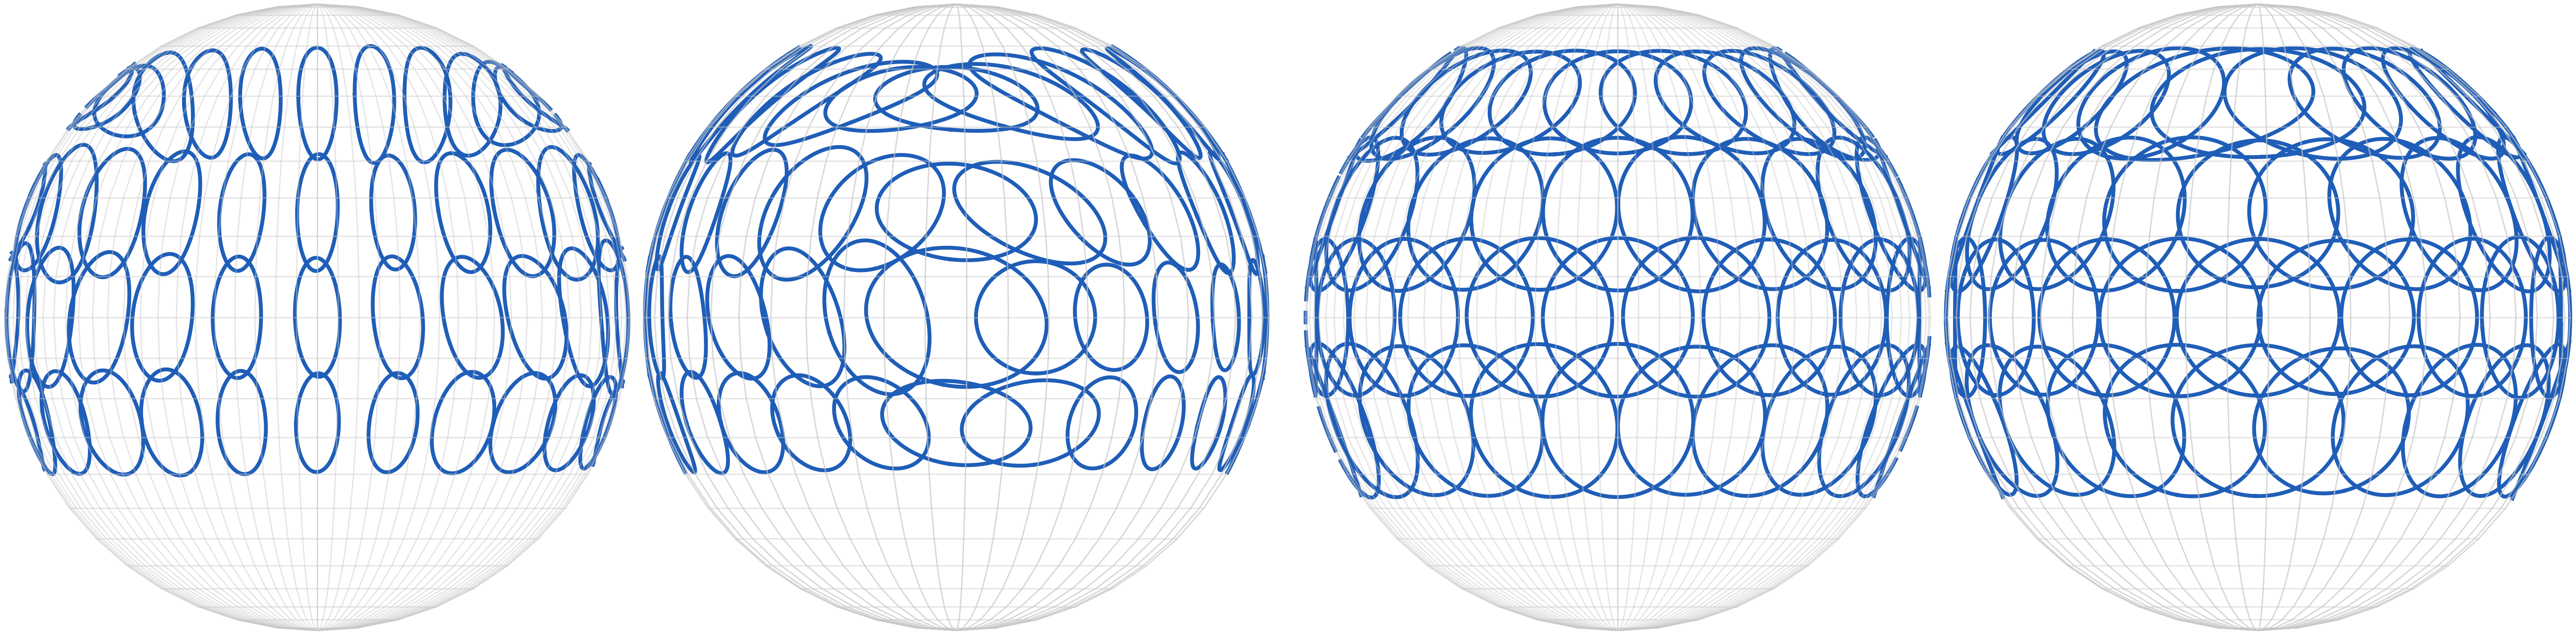
\includegraphics[width=\textwidth]{figures/ellipse_comparison.png}
    \caption[Fisher discrimination ellipses and Barumerli response covariance]{Left pair: local discrimination ellipses from the Cram\'er--Rao bound, i.e.\ the inverse of the elementwise median Fisher tensor of the 41 evaluation subjects (dense measured HRTFs), drawn as 95\% contours (\(\sqrt{\chi^2_{2,0.95}}\approx2.45\) times the \(d'=1\) ellipse) for visibility. Right pair: one-standard-deviation ellipses of the elementwise median local response covariance of the Barumerli MAP observer~\cite{Barumerli2023}, from 300 simulated responses per direction and subject, excluding non-local responses (great-circle error \(\ge45^\circ\)). The two halves are drawn at different scales, so ellipse sizes should not be compared directly. Each pair shows views from the front (azimuth \(0^\circ\)) and from the left (azimuth \(90^\circ\)), in the same tangent basis.}
    \label{fig:sonicom_kent}
\end{figure*}

\section{AIRM Tensor Discrepancy}
The target and reconstructed tensors are compared using the affine-invariant Riemannian metric (AIRM) on symmetric positive-definite (SPD) matrices, chosen for three properties. It is invariant under congruence, \(\mathbf g\mapsto\mathbf A^T\mathbf g\mathbf A\) for invertible \(\mathbf A\), so it does not depend on the tangent basis or on a common rescaling of the cue noise. It depends only on ratios of sensitivity, so halving and doubling discriminability are penalised equally. And it is sensitive to changes in the size, anisotropy, and orientation of the discrimination ellipse.

AIRM requires strictly positive-definite arguments, whereas a Fisher tensor is singular wherever the weighted cue gradients fail to span both tangent directions. Both tensors are therefore symmetrised and regularised by the same isotropic term, \(\mathbf{g}_{\eta}=\mathbf{g}+\eta\mathbf{I}_2\) and \(\widehat{\mathbf{g}}_{\eta}=\widehat{\mathbf{g}}+\eta\mathbf{I}_2\), with \(\eta=10^{-6}\,\mathrm{rad}^{-2}\). By \eqref{eq:threshold}, \(\eta\) alone corresponds to a \(d'=1\) displacement of \(10^3\) rad, far larger than any angle on the sphere, so the regularisation affects only directions along which the cues carry effectively no information. Directions at which the smallest eigenvalue of either tensor falls below \(100\eta\) are counted as near-singular and reported separately. The pointwise discrepancy is
\begin{equation}
 d_{\mathrm{AIRM}}
 =
 \left\|\log\!\left(
 \mathbf{g}_{\eta}^{-1/2}
 \widehat{\mathbf{g}}_{\eta}
 \mathbf{g}_{\eta}^{-1/2}
 \right)\right\|_F
 =\sqrt{\log^2\lambda_1+\log^2\lambda_2},
\end{equation}
where \(\lambda_1\ge\lambda_2>0\) are the generalised eigenvalues of \((\widehat{\mathbf{g}}_{\eta},\mathbf{g}_{\eta})\), solving \(\widehat{\mathbf g}_\eta\mathbf v=\lambda\,\mathbf g_\eta\mathbf v\). They are computed from the Cholesky factor \(\mathbf g_\eta=\mathbf L\mathbf L^T\) as the eigenvalues of \(\mathbf L^{-1}\widehat{\mathbf g}_{\eta}\mathbf L^{-T}\), floored at \(10^{-12}\); non-finite tensors are rejected rather than floored.

These eigenvalues have a direct discriminability interpretation. They are the extrema over displacement directions \(\mathbf u\) of the Rayleigh quotient
\begin{equation}
\frac{\mathbf u^T\widehat{\mathbf g}_{\eta}\mathbf u}{\mathbf u^T\mathbf g_{\eta}\mathbf u}
=
\left(\frac{\widehat{d}'}{d'}\right)^{2}
=
\left(\frac{\rho_{d'=1}}{\widehat{\rho}_{d'=1}}\right)^{2},
\end{equation}
where hats denote the reconstruction and \(d'\) is evaluated for a fixed displacement \(\rho\mathbf u\). Writing \(\kappa_i=\sqrt{\lambda_i}\), \(d_{\mathrm{AIRM}}=2\sqrt{\log^2\kappa_1+\log^2\kappa_2}\), where \(\kappa_1\) and \(\kappa_2\) are the largest and smallest factors by which the reconstruction scales the predicted \(d'\) for a fixed angular displacement, and their reciprocals the factors by which it scales the local \(d'=1\) threshold. AIRM therefore measures predicted discriminability change directly within the observer model. For example, a discrepancy of \(0.5\) along one principal direction, with the orthogonal direction unchanged, corresponds to a threshold change by a factor of \(e^{0.25}\approx1.28\). A uniform change in discriminability gives \(\lambda_1=\lambda_2\neq1\), whereas a change in anisotropy or orientation alone gives \(\lambda_1\lambda_2=1\) with \(\lambda_1\neq\lambda_2\). The discrepancy is zero only if the two ellipses are identical. The mean discrepancy over the evaluation grid \(\{\mathbf r_n\}_{n=1}^{N_{\mathrm{eval}}}\) is
\begin{equation}
\mathcal{E}_{\mathrm{AIRM}} =
\frac{1}{N_{\mathrm{eval}}}\sum_{n=1}^{N_{\mathrm{eval}}}
 d_{\mathrm{AIRM}}\bigl(\mathbf g_\eta(\mathbf r_n),
 \widehat{\mathbf g}_\eta(\mathbf r_n)\bigr).
\label{eq:mean_airm}
\end{equation}
The 793-direction SONICOM grid is not equal-area, so this unweighted mean gives more weight to densely sampled regions; it is used for consistency with the direction-averaged signal metrics.

\section{Evaluation Metrics}
Three families of metrics are reported. Signal-domain metrics measure physical reconstruction error at each direction, the Fisher-tensor metrics measure whether the local discriminability implied by the cue field is preserved, and the Bayesian-observer metrics summarise simulated localisation performance. The first and third are established in the upsampling literature and serve as context for the second.

\subsection{Signal-Domain Metrics}
The binaural log-spectral distortion over the \(W\) frequency bins \(f_w\) of the evaluation band is
\begin{equation}
\operatorname{LSD}
=\frac{1}{2N_{\mathrm{eval}}}
\sum_{n,c}\Biggl[
\frac{1}{W}\sum_{w=1}^{W}
\left(
20\log_{10}
\frac{A_c(f_w,\mathbf{r}_n)}
{\widehat{A}_c(f_w,\mathbf{r}_n)}
\right)^2\Biggr]^{1/2},
\end{equation}
with magnitudes floored at \(10^{-8}\). LSD is computed on HRTF rather than DTF magnitudes, so it includes direction-independent errors that the cue analysis removes. The evaluation band is 20~Hz to 16~kHz for every method; the conventional 20-kHz band is recorded in the released results but is not comparable across methods, because FSP-AE has no output above 16~kHz. The ILD error \(\mathcal E_{\mathrm{ILD}}\) is the mean absolute difference over directions between the reference and reconstructed ILDs of \eqref{eq:ild}, computed on the band-limited HRIRs \(a_c\) rather than on DTFs, following the SAM/LAP convention.

\subsection{Fisher-Tensor Metrics}
The primary tensor metric is \(\mathcal E_{\mathrm{AIRM}}\) \eqref{eq:mean_airm}. To show which ellipse property drives it, three summaries are added. Let \(\nu_1(\mathbf{r})\geq\nu_2(\mathbf{r})>0\) be the eigenvalues of \(\mathbf{g}_{\eta}(\mathbf{r})\), and \(\mathbf{v}_1(\mathbf{r})\) the principal information direction, along which discrimination is finest. Then
\begin{align}
\mathcal{E}_{\mathrm{det}} &=
\frac{1}{N_{\mathrm{eval}}}\sum_n
\left|\log\frac{\det\widehat{\mathbf{g}}_{\eta}(\mathbf{r}_n)}
{\det\mathbf{g}_{\eta}(\mathbf{r}_n)}\right|, \\
\mathcal{E}_{\mathrm{anis}} &=
\frac{1}{N_{\mathrm{eval}}}\sum_n
\left|\log\frac{\hat{\nu}_1(\mathbf{r}_n)/\hat{\nu}_2(\mathbf{r}_n)}
{\nu_1(\mathbf{r}_n)/\nu_2(\mathbf{r}_n)}\right|, \\
\mathcal{E}_{\mathrm{orient}} &=
\frac{1}{|\mathcal{R}_{\mathrm{aniso}}|}
\sum_{\mathbf{r}_n\in\mathcal{R}_{\mathrm{aniso}}}
\arccos
\left|\widehat{\mathbf{v}}_1(\mathbf{r}_n)^T\mathbf{v}_1(\mathbf{r}_n)\right|.
\end{align}
Since ellipse area scales as \((\det\mathbf g)^{-1/2}\), \(\mathcal E_{\mathrm{det}}\) measures change in overall scale, \(\mathcal E_{\mathrm{anis}}\) change in elongation independently of scale, and \(\mathcal E_{\mathrm{orient}}\) rotation of the principal axes (degrees, \(0\)--\(90^\circ\)). Orientation is undefined for an isotropic tensor, so \(\mathcal E_{\mathrm{orient}}\) is restricted to the set \(\mathcal{R}_{\mathrm{aniso}}\) of directions at which both tensors satisfy \(\nu_1/\nu_2\geq1.10\). The signed counterpart of \(\mathcal E_{\mathrm{det}}\), without the absolute value, shows whether a reconstruction adds or removes information. All summaries are invariant to the choice of tangent basis.

\subsection{Bayesian Localisation Metrics}\label{sec:bayes}
Localisation is simulated with the Bayesian observer of Barumerli et al.~\cite{Barumerli2023} (AMT \path{barumerli2023}) with band-level spectral features (AMT \path{dtf}), the common 16-kHz cue band, and MAP estimation. The observer's template is built from the measured reference HRTFs and held fixed, while the targets are rendered with the HRTF set under evaluation. This models a listener whose templates were learned from their own ears and who is presented with reconstructed cues. A dense self-reference condition, with targets also rendered from the measured HRTFs, provides the baseline. The template uses the AMT~1.6 interpolation, which omits directions below the lowest measured elevation; a later full-sphere extension removes this limitation~\cite{Barumerli2026}.

Each target direction is simulated 300 times. Following Middlebrooks~\cite{Middlebrooks1999}, as implemented in AMT \path{barumerli2023_metrics}, the lateral RMS error is computed over all trials. Polar errors are evaluated on the subset \(\mathcal P\) of trials whose responses lie within \(30^\circ\) of the median plane, and a response is local if its wrapped polar error is below \(90^\circ\). The local polar RMS error is computed over the local subset \(\mathcal A\subseteq\mathcal P\), and the quadrant error is \((1-|\mathcal A|/|\mathcal P|)\times100\%\). The model parameters are \(\sigma_{\mathrm{ITD}}=0.569\) JND units, \(\sigma_{\mathrm{ILD}}=1\)~dB, \(\sigma_{\mathrm{spectral}}=4\)~dB, \(\sigma_{\mathrm{prior}}=11.5^\circ\), and \(\sigma_{\mathrm{motor}}=14^\circ\). The band-level features, MAP estimation, and \(\sigma_{\mathrm{spectral}}\) follow the localisation evaluation of Hogg et al.~\cite{Hogg2024GAN} used in SONICOM upsampling studies; the remaining parameters, including \(\sigma_{\mathrm{motor}}\), are the AMT~1.6 defaults. Metrics are reported as differences from the dense self-reference of the same subject.

The two cue-based analyses ask different questions. The Bayesian metrics measure how well a reconstruction matches the listener's reference templates; the Fisher tensor measures whether the reconstructed cue field retains the local gradient structure on which discrimination depends, independently of any template.

\section{Evaluation Procedure}
\subsection{Data and Spatial Conditions}\label{sec:data}
The evaluation uses the 48-kHz \path{FreeFieldCompMinPhase} version of the SONICOM HRTF dataset~\cite{Engel2023}. Here, \emph{MinPhase} refers to the minimum-phase inverse filter used for free-field compensation, not to a minimum-phase reconstruction of each HRTF; the measured HRIRs retain their interaural delays. The neural methods are trained on 162 subjects, and all methods are evaluated on the same 41 held-out subjects. The subject split and sparse masks follow the SONICOM upsampling protocol used by Hu et al.\ for HRTFformer, within the broader LAP upsampling benchmark~\cite{Hu2026HRTFformer,Hogg2025LAPUpsampling}.

Four sparse-to-dense conditions are evaluated: \(100\rightarrow793\), \(19\rightarrow793\), \(5\rightarrow793\), and \(3\rightarrow793\). Within each condition, the same retained directions are used for every method and subject (Fig.~\ref{fig:sampling_scheme}). Each reconstruction is evaluated on the full dense grid, including the retained directions, and measured HRIRs are not substituted at the retained nodes. The grid contains no duplicate directions. A 512-point FFT gives 256 non-DC bins per ear.

\begin{figure}[t]
    \centering
    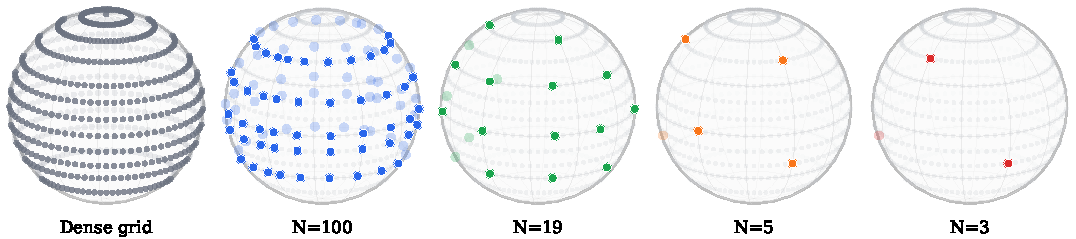
\includegraphics[width=\columnwidth]{figures/sampling_scheme_overview.pdf}
    \caption[Dense and sparse SONICOM sampling schemes]{Dense SONICOM evaluation grid and retained sparse sampling schemes used for the four upsampling conditions. Grey points denote the dense 793-direction target grid; coloured points denote retained directions.}
    \label{fig:sampling_scheme}
\end{figure}

\subsection{Compared Reconstruction Methods}
Two families of methods are compared. The SUpDEq configurations follow the directional equalisation approach of P\"orschmann et al.~\cite{Poerschmann2019SUpDEq}, in which HRTFs are equalised by a rigid-sphere model before spatial interpolation and de-equalised afterwards: \textbf{SUpDEq-SH} uses SH interpolation; \textbf{SUpDEq-MCA}, the distributed magnitude-corrected configuration, adds magnitude correction with unlimited boost; and \textbf{SUpDEq-Natural-MCA} and \textbf{SUpDEq-Bary-MCA} replace SH interpolation by natural-neighbour (Voronoi-weighted, as in the SFS/SUpDEq routines) or barycentric interpolation, with boosts limited to 6~dB. The neural methods are \textbf{RANF}, a retrieval-augmented neural field that predicts magnitude and ITD and reconstructs HRIRs from a minimum-phase representation with ITD compensation~\cite{Masuyama2025RANF,Masuyama2025ICASSPRANF}, and \textbf{FSP-AE}, a network conditioned on source position and frequency that predicts magnitude and ITD before HRIR reconstruction~\cite{Ito2025FSPAE}, generated at 32~kHz and resampled to 48~kHz.

For the SH-based SUpDEq configurations, the interpolation order is capped at \(\min(6,\lfloor\sqrt{N_{\mathrm{ret}}}\rfloor-1)\) for \(N_{\mathrm{ret}}\) retained directions, giving orders 6, 3, 1, and 0 for the four conditions. At \(N_{\mathrm{ret}}=3\), the interpolated equalised field is therefore direction-independent, and the remaining directional variation comes only from the rigid-sphere de-equalisation.

Two interpolation stages are undefined at the sparsest grids, and these conditions are reported as not applicable rather than scored. Barycentric interpolation requires every target direction to lie within a triangle of the convex hull of the retained directions, which holds only if the hull encloses the listener. Three directions cannot form such a hull, and the five retained directions of the \(N=5\) mask, all in the frontal hemisphere, do not enclose it either. Natural-neighbour interpolation fails at \(N=5\) and \(N=3\) because the spherical Voronoi weights are undefined for these configurations, and the SUpDEq magnitude-correction stage rejects the resulting undefined values. Every reconstruction is also checked for non-finite or all-zero HRIRs before evaluation.

\subsection{Preprocessing}
Methods operating in the SH domain are inverse-transformed to HRIRs on the dense grid, so every method yields a dense HRIR set, from which magnitudes are obtained by a common FFT. Fisher and observer cues are extracted from every method's HRIRs with the same band limit, CTF procedure, and feature conventions. For RANF and FSP-AE, the model-predicted ITD is therefore embedded in the generated HRIRs and re-estimated in the same way as for all other methods, rather than taken from the model output.
\section{Results}
\subsection{Evaluation Coverage}
Of the 984 subject--method--condition combinations (41 subjects, four retention levels, six methods), 164 are not applicable: SUpDEq-Bary-MCA and SUpDEq-Natural-MCA at \(N=5\) and \(N=3\) (Section~\ref{sec:data}). The remaining 820, across 20 method--retention conditions, were evaluated with all metrics; none contained non-finite or all-zero HRIRs.

\begin{figure}[!t]
    \centering
    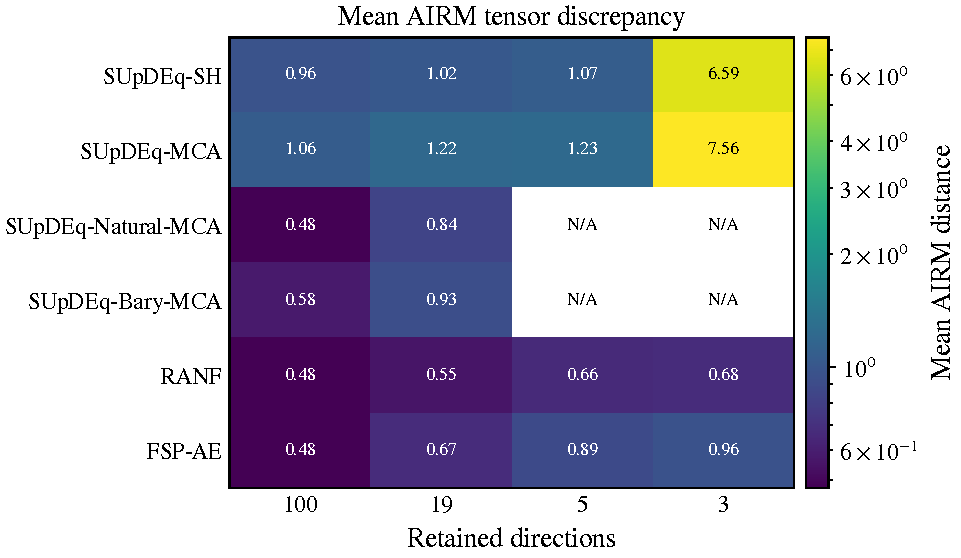
\includegraphics[width=\columnwidth]{figures/airm_heatmap.pdf}
    \caption[Mean AIRM discrepancy over methods and retention conditions]{Mean Fisher-tensor AIRM discrepancy over the 41-subject cohort. Lower values indicate closer preservation of the dense-reference tensor field. N/A marks conditions in which the interpolation stage is undefined.}
    \label{fig:airm_heatmap}
\end{figure}

\subsection{Fisher-Tensor Results}
Figure~\ref{fig:airm_heatmap} reports the cohort-mean AIRM discrepancy, which measures how far each reconstruction alters the local discrimination ellipses of the dense reference. RANF gives the lowest mean AIRM at \(N=19\), \(N=5\), and \(N=3\) (0.55, 0.66, and 0.68), followed in each case by FSP-AE (0.67, 0.89, and 0.96). At \(N=100\), SUpDEq-Natural-MCA, FSP-AE, and RANF are effectively tied (0.476, 0.476, and 0.477), and SUpDEq-Bary-MCA follows at 0.58. The SH-based SUpDEq configurations are the least faithful at every retention level. At \(N=3\), where their interpolation order is zero, SUpDEq-SH and SUpDEq-MCA reach mean AIRM values of 6.6 and 7.6. This reflects a loss of local cue structure over most of the sphere rather than a few extreme directions: the median pointwise discrepancy is 6.3 and 7.2, and only 2.9\% of directions are near-singular. No other condition contains near-singular directions.

\begin{table*}[!t]
\centering
\caption{Cohort-mean Fisher-tensor component errors: \(\mathcal E_{\mathrm{det}}\) (det), \(\mathcal E_{\mathrm{anis}}\) (anis), and \(\mathcal E_{\mathrm{orient}}\) (orient., degrees). Signed: mean signed log ratio \(\log\det\widehat{\mathbf g}_\eta-\log\det\mathbf g_\eta\) over directions and subjects; negative values indicate lost discriminability (ellipse area scales by \(e^{-x/2}\)), positive values spurious added cue variation. In parentheses: percentage of directions at which the reconstruction carries more information than the reference. N/A: not applicable.}
\label{tab:tensor_component_means}
\scriptsize
\setlength{\tabcolsep}{2.4pt}
\begin{tabular}{lrrrrrrrrrrrrrrrr}
\toprule
 & \multicolumn{4}{c}{\(N=100\)} & \multicolumn{4}{c}{\(N=19\)} & \multicolumn{4}{c}{\(N=5\)} & \multicolumn{4}{c}{\(N=3\)} \\
\cmidrule(lr){2-5} \cmidrule(lr){6-9} \cmidrule(lr){10-13} \cmidrule(lr){14-17}
Method & det & anis & orient. & signed & det & anis & orient. & signed & det & anis & orient. & signed & det & anis & orient. & signed \\
\midrule
SUpDEq-SH & 0.70 & 0.56 & 19 & +0.50 (72\%) & 0.68 & 0.67 & 20 & +0.46 (73\%) & 0.87 & 0.67 & 16 & \(-\)0.52 (31\%) & 7.05 & 5.72 & 13 & \(-\)7.05 (0\%) \\
SUpDEq-MCA & 0.90 & 0.57 & 19 & +0.80 (81\%) & 0.93 & 0.68 & 22 & +0.83 (85\%) & 0.96 & 0.81 & 17 & \(-\)0.66 (27\%) & 8.45 & 6.17 & 13 & \(-\)8.45 (0\%) \\
SUpDEq-Natural-MCA & 0.33 & 0.32 & 7 & \(-\)0.14 (36\%) & 0.70 & 0.55 & 11 & \(-\)0.49 (29\%) & \multicolumn{4}{c}{N/A} & \multicolumn{4}{c}{N/A} \\
SUpDEq-Bary-MCA & 0.38 & 0.39 & 9 & \(-\)0.18 (33\%) & 0.68 & 0.55 & 14 & \(-\)0.35 (36\%) & \multicolumn{4}{c}{N/A} & \multicolumn{4}{c}{N/A} \\
RANF & 0.35 & 0.33 & 7 & \(-\)0.05 (50\%) & 0.39 & 0.37 & 9 & +0.01 (53\%) & 0.48 & 0.44 & 11 & \(-\)0.05 (48\%) & 0.50 & 0.45 & 11 & \(-\)0.12 (43\%) \\
FSP-AE & 0.37 & 0.32 & 7 & \(-\)0.24 (29\%) & 0.60 & 0.44 & 8 & \(-\)0.54 (14\%) & 0.86 & 0.58 & 10 & \(-\)0.83 (6\%) & 0.95 & 0.63 & 10 & \(-\)0.93 (4\%) \\
\bottomrule
\end{tabular}
\end{table*}


Table~\ref{tab:tensor_component_means} decomposes the discrepancy into errors in tensor scale, anisotropy, and principal-axis orientation. The learning-based methods and the natural-neighbour and barycentric variants have orientation errors of 7--14\(^\circ\), whereas the SH-based SUpDEq configurations rotate the principal axes by 16--22\(^\circ\) on average at \(N\ge5\). The scale error also has a sign, which no direction-wise spectral error can reveal (signed columns of Table~\ref{tab:tensor_component_means}). RANF is unbiased at every retention level: about half the directions gain and half lose information. FSP-AE and the natural-neighbour and barycentric variants systematically reduce Fisher information, as expected of reconstructions that smooth the cue field. For FSP-AE this grows with sparsity, from \(-0.24\) at \(N=100\) to \(-0.93\) at \(N=3\), equivalent to discrimination ellipses \(e^{0.93/2}\approx1.6\) times larger in area than those of the measured HRTFs. In contrast, SUpDEq-SH and SUpDEq-MCA at \(N=100\) and \(N=19\) increase the Fisher information at 72--85\% of directions. This indicates spurious cue variation, which would support finer discrimination only for an observer adapted to the reconstructed field, not for a listener whose templates come from their own ears (Section~\ref{sec:discussion}).

\subsection{Robustness of the Tensor Ranking}\label{sec:sensitivity}
Every tensor was recomputed from the stored per-cue-family Gram matrices with all else held fixed (Table~\ref{tab:sensitivity}). Refitting the cue fields at SH orders 4 and 8, and increasing the spectral noise from \(\sigma_{\mathrm{mon}}=1.25\) to 2.85~dB (the value estimated for SONICOM listeners, Section~\ref{sec:discussion}), left the complete ranking unchanged at \(N=19\), \(N=5\), and \(N=3\). At \(N=100\), the three leading methods remain within 0.1 of one another and their order changes with the settings, so no distinction is drawn between them. SUpDEq-Bary-MCA, SUpDEq-SH, and SUpDEq-MCA rank below them under every setting except SH order 8, where SUpDEq-Bary-MCA moves ahead of RANF and FSP-AE.

\begin{table}[!t]
\centering
\caption{Method ranking by cohort-mean AIRM (best first) under the primary settings and under changes to the SH order of the cue fit and to the spectral noise weight, over the methods applicable at each retention level. All settings: the ranking is identical under all four.}
\label{tab:sensitivity}
\scriptsize
\setlength{\tabcolsep}{2.5pt}
\begin{tabular}{rll}
\toprule
$N$ & Setting & Ranking \\
\midrule
100 & Primary & Nat \(<\) FSP \(<\) RANF \(<\) Bary \(<\) SH \(<\) MCA \\
 & SH order 4 & FSP \(<\) RANF \(<\) Nat \(<\) Bary \(<\) SH \(<\) MCA \\
 & SH order 8 & Nat \(<\) Bary \(<\) RANF \(<\) FSP \(<\) MCA \(<\) SH \\
 & \(\sigma_{\mathrm{mon}}=2.85\)~dB & RANF \(<\) FSP \(<\) Nat \(<\) Bary \(<\) SH \(<\) MCA \\
\addlinespace
19 & All settings & RANF \(<\) FSP \(<\) Nat \(<\) Bary \(<\) SH \(<\) MCA \\
\addlinespace
5 & All settings & RANF \(<\) FSP \(<\) SH \(<\) MCA \\
\addlinespace
3 & All settings & RANF \(<\) FSP \(<\) SH \(<\) MCA \\
\bottomrule
\end{tabular}
\end{table}


\subsection{Signal and Bayesian-Observer Metrics}
RANF has the lowest LSD in every retention condition (2.8--4.2~dB over 20~Hz--16~kHz). FSP-AE has higher LSD than RANF and than the natural-neighbour and barycentric variants at \(N=100\), but its LSD increases only from 3.9 to 4.9~dB between \(N=100\) and \(N=3\). The SH-based SUpDEq configurations have the highest LSD at every retention level.


Figure~\ref{fig:bayesian_subject_distributions} shows the Bayesian-observer degradation relative to the dense self-reference. RANF has the smallest local polar degradation at every retention level (0.9--3.6\(^\circ\)), and SUpDEq-SH the largest at \(N\ge5\) (5.7--16.6\(^\circ\)), with quadrant-error increases of 14--51 percentage points (pp). Magnitude correction reduces both at \(N\ge5\), most strongly the quadrant error (by 9, 33, and 32~pp at \(N=100\), 19, and 5), but at \(N=3\) the two SH-based configurations are equally degraded and SUpDEq-MCA adds a \(13.7^\circ\) lateral error. Quadrant error separates the neural methods differently from the other metrics: it increases by 2.7--6.5~pp for FSP-AE but by 5.0--11.5~pp for RANF.

\begin{figure}[!t]
    \centering
    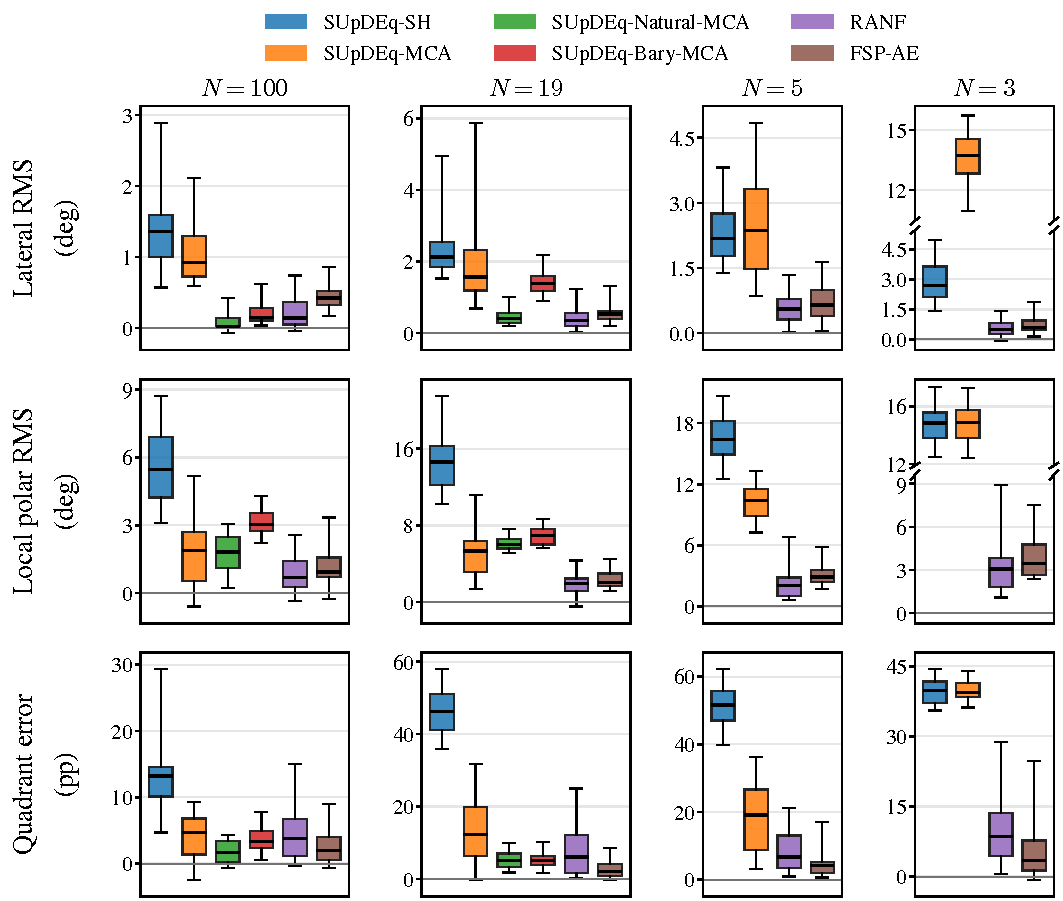
\includegraphics[width=\columnwidth]{figures/bayesian_subject_boxplots.pdf}
    \caption[Subject-wise Bayesian-observer distribution summaries]{Subject-wise Bayesian-observer degradation over the 41 held-out subjects, relative to the dense self-reference. Boxes show medians and interquartile ranges; whiskers span the 5th--95th percentiles. Each panel has its own vertical scale, broken only across ranges that contain no data; not-applicable conditions are omitted.}
    \label{fig:bayesian_subject_distributions}
\end{figure}

\subsection{Metric Relationships}
Figure~\ref{fig:metric_relationships} plots AIRM against LSD and relative local polar RMS. The rows form a repeated subject--method--condition design, so they are not treated as independent samples and no \(p\)-values are computed. Table~\ref{tab:metric_correlations} reports three levels of association: across the 20 method--retention means, across all rows with 95\% intervals from 1,000 resamples of subjects, and within each subject and retention level.

The across-condition association with LSD is strong (Spearman 0.92). Much of it is expected, because all metrics worsen as retention decreases. Agreement across conditions therefore does not imply that the metrics agree on which method best preserves discrimination at a given retention level. Within conditions, the rank agreement between AIRM and LSD falls to a Kendall \(\tau\) of 0.73 [0.71, 0.74], and to 0.56 [0.53, 0.58] for ILD error. The Bayesian metrics show the same pattern: across conditions, their Spearman correlations with AIRM are 0.95 (lateral), 0.83 (local polar), and 0.75 (quadrant), but the within-condition agreement falls to 0.65, 0.56, and 0.39.

The departures are concentrated in specific method pairs, where the tensor analysis adds information. Three are consistent across subjects. First, magnitude correction lowers LSD relative to SUpDEq-SH by 1.1, 4.3, and 2.0~dB at \(N=100\), 19, and 5, for at least 95\% of subjects. Yet it increases the AIRM discrepancy for 80\%, 98\%, and 85\% of subjects, mainly through the scale component (Table~\ref{tab:tensor_component_means}); at \(N=100\) and \(N=19\) the corrected magnitudes add further spurious direction-to-direction cue variation to that already introduced by SH interpolation (signed columns). Second, at \(N=100\) SUpDEq-Natural-MCA and SUpDEq-Bary-MCA have the same mean LSD (3.24~dB), but the barycentric variant has the larger AIRM for 95\% of subjects (0.58 against 0.48), mainly through greater anisotropy and orientation errors. Third, FSP-AE has higher LSD than SUpDEq-Bary-MCA at \(N=100\) for every subject (3.88 against 3.24~dB), yet lower AIRM for 98\% of them. At \(N=19\), FSP-AE also has a larger broadband ILD error than SUpDEq-Natural-MCA for 98\% of subjects (1.85 against 1.12~dB), yet a smaller AIRM for 98\%. The Bayesian observer sides with LSD in the first case: SUpDEq-MCA has lower local polar and quadrant degradation than SUpDEq-SH for at least 98\% of subjects at \(N=100\), 19, and 5. In the second and third it sides with AIRM: SUpDEq-Bary-MCA has larger local polar degradation than SUpDEq-Natural-MCA for 98\% of subjects and than FSP-AE for 93\% at \(N=100\), and SUpDEq-Natural-MCA larger than FSP-AE for every subject at \(N=19\). A fourth disagreement involves the leading neural methods: at \(N\le19\), RANF has lower AIRM than FSP-AE for at least 93\% of subjects, but a larger quadrant-error increase for 68--78\% of them.

\begin{table}[!t]
\centering
\caption{Rank association between mean AIRM and the other metrics. Across conditions: Spearman correlation of the method--retention means. Row-wise: Spearman correlation over all subject--method--retention rows, with 95\% subject-bootstrap intervals. Within condition: Kendall's \(\tau\) between the method rankings given by AIRM and by the metric, computed separately for each subject and retention level and averaged, with 95\% subject-bootstrap intervals; it excludes agreement that arises only because all metrics worsen with sparsity.}
\label{tab:metric_correlations}
\scriptsize
\setlength{\tabcolsep}{3pt}
\begin{tabular}{lrrr}
\toprule
Metric & Across cond. & Row-wise & Within cond. \(\tau\) \\
\midrule
LSD & 0.92 & 0.87 [0.86, 0.89] & 0.73 [0.71, 0.74] \\
ILD & 0.77 & 0.74 [0.72, 0.76] & 0.56 [0.53, 0.58] \\
Lateral RMS & 0.95 & 0.82 [0.80, 0.84] & 0.65 [0.62, 0.67] \\
Local polar RMS & 0.83 & 0.71 [0.67, 0.75] & 0.56 [0.53, 0.59] \\
Quadrant error & 0.75 & 0.58 [0.53, 0.62] & 0.39 [0.35, 0.44] \\
\bottomrule
\end{tabular}
\end{table}


\begin{figure}[!t]
    \centering
    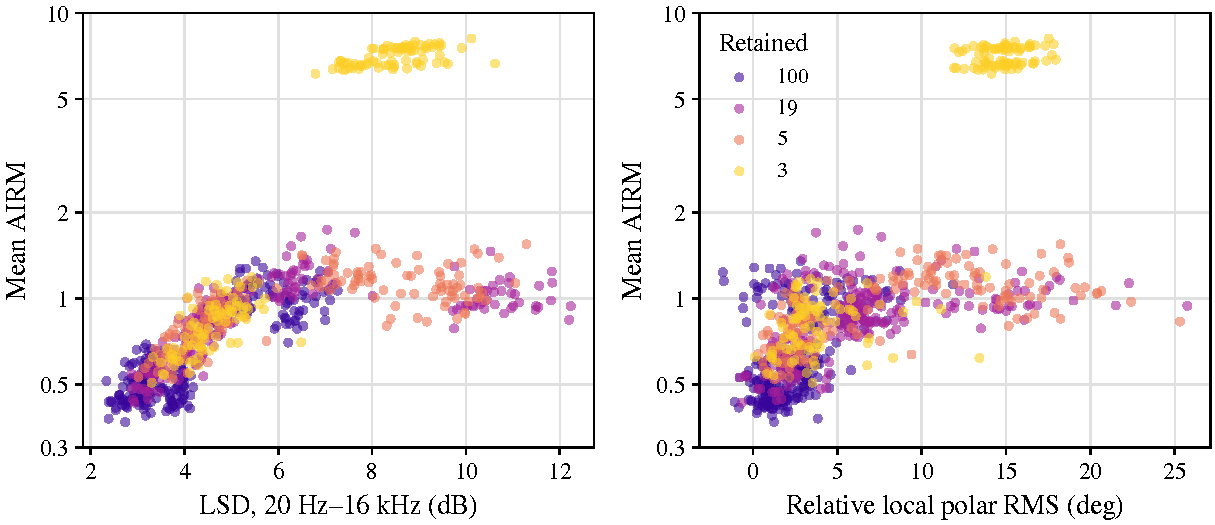
\includegraphics[width=\columnwidth]{figures/metric_relationships_paper.pdf}
    \caption[Relationships between AIRM and other evaluation metrics]{Mean AIRM discrepancy (log scale) against LSD (20~Hz--16~kHz) and relative local polar RMS for every evaluated subject--method--condition row, coloured by retention level. Association summaries are reported in Table~\ref{tab:metric_correlations}.}
    \label{fig:metric_relationships}
\end{figure}

\subsection{Local Discrimination-Threshold Plausibility}\label{sec:thresholds}
To express the tensors in a psychophysical unit, and to check that the observer model predicts discrimination on a realistic scale, the \(d'=1\) threshold \eqref{eq:threshold} was evaluated for each subject along selected tangent directions. Horizontal thresholds were computed along the azimuthal tangent at \((0^\circ,0^\circ)\), \((45^\circ,0^\circ)\), and \((90^\circ,0^\circ)\), and vertical thresholds along the elevational tangent at \((0^\circ,0^\circ)\) and \((0^\circ,45^\circ)\), where coordinate pairs denote azimuth and elevation. An oblique threshold was computed in front along the direction \(60^\circ\) from horizontal. Table~\ref{tab:local_threshold_plausibility} reports cohort medians. No parameter was fitted to the behavioural data below.

\begin{table}[!t]
\centering
\caption{Cohort-median Fisher-predicted \(d'=1\) thresholds in degrees. Coordinate pairs give (azimuth, elevation); H and V are horizontal (azimuthal) and vertical (elevational) displacements, and D is the oblique displacement at \(60^\circ\) from horizontal. Err.\ is the mean absolute log ratio to the dense reference over the six thresholds, expressed as a percentage change.}
\label{tab:local_threshold_plausibility}
\scriptsize
\setlength{\tabcolsep}{2.2pt}
\resizebox{\columnwidth}{!}{%
\begin{tabular}{llrrrrrrr}
\toprule
Method & $N$ & H\,(0,0) & H\,(45,0) & H\,(90,0) & V\,(0,0) & V\,(0,45) & D\,(0,0) & Err. \\
\midrule
Measured & -- & 1.69 & 3.06 & 6.83 & 4.47 & 5.99 & 2.73 & -- \\
Measured, \(\sigma_{\mathrm{mon}}=2.85\) & -- & 1.70 & 3.34 & 10.97 & 9.17 & 11.64 & 3.06 & -- \\
SUpDEq-SH & 19 & 2.06 & 2.93 & 5.50 & 4.13 & 3.94 & 3.03 & 19\% \\
SUpDEq-MCA & 19 & 1.86 & 2.56 & 5.75 & 4.25 & 5.15 & 3.04 & 13\% \\
SUpDEq-Natural-MCA & 19 & 1.88 & 2.86 & 6.31 & 6.06 & 7.10 & 3.48 & 18\% \\
SUpDEq-Bary-MCA & 19 & 1.83 & 3.05 & 5.88 & 6.25 & 7.17 & 3.40 & 18\% \\
RANF & 19 & 1.67 & 2.94 & 6.64 & 4.34 & 6.35 & 2.74 & 3\% \\
FSP-AE & 19 & 1.79 & 3.42 & 8.34 & 4.83 & 7.16 & 2.88 & 12\% \\
SUpDEq-SH & 5 & 1.96 & 2.88 & 5.44 & 5.47 & 5.01 & 3.29 & 18\% \\
SUpDEq-MCA & 5 & 1.65 & 2.61 & 5.55 & 6.82 & 6.08 & 2.99 & 16\% \\
RANF & 5 & 1.76 & 3.05 & 7.72 & 4.28 & 7.05 & 2.86 & 7\% \\
FSP-AE & 5 & 1.71 & 3.35 & 10.24 & 6.50 & 9.89 & 3.14 & 29\% \\
\bottomrule
\end{tabular}%
}
\end{table}


Measured minimum audible angles are defined at a percent-correct criterion, whereas the predictions are \(d'=1\) thresholds. Converting between the two requires a model of the listener's task and decision process, but any criterion common to one study cancels in a ratio, so predictions are compared with ratios measured within the same study; absolute values indicate scale only. The dense reference predicts horizontal thresholds of \(1.69^\circ\), \(3.06^\circ\), and \(6.83^\circ\) at \(0^\circ\), \(45^\circ\), and \(90^\circ\) azimuth, ratios of 1.82 and 4.05 to the frontal value. Stevenson-Hoare reports horizontal-plane means, collapsed over left and right, of approximately \(1.5^\circ\), \(2.7^\circ\), and \(7.2^\circ\), ratios of 1.8 and 4.8~\cite{StevensonHoare2020}. In front, the predicted vertical threshold (\(4.47^\circ\)) exceeds the horizontal one by a factor of 2.7, and grows to \(5.99^\circ\) at \(45^\circ\) elevation. Grantham et al.\ report the same ordering for wideband noise in front, with \(1.6^\circ\) horizontally and \(6.5^\circ\) vertically, a ratio of 4.1~\cite{Grantham2003}. They also measured a \(60^\circ\) diagonal trajectory, which neither axis threshold determines alone: the tensor predicts \(2.73^\circ\) (interquartile range \(2.52\)--\(2.95^\circ\) across subjects), 1.62 times the horizontal threshold, against a measured ratio of 1.75. The ratios involving elevation depend most on the spectral weight. With the SONICOM estimate \(\sigma_{\mathrm{mon}}=2.85\)~dB, the vertical-to-horizontal ratio rises to 5.4 and the diagonal ratio to 1.80, so both measured ratios, and the \(90^\circ\)-to-\(0^\circ\) horizontal ratio (4.1 and 6.4 against 4.8), lie between the predictions of the two calibrations. The tensor therefore reproduces the directional pattern of measured frontal spatial acuity, and the spectral noise weight determines where within this range it falls. These thresholds are defined at the spatial scale of the order-6 cue fit, roughly $18^\circ$. Thresholds dominated by spectral cues decrease with fit order (frontal vertical: $6.0^\circ$, $4.5^\circ$, and $3.6^\circ$ at orders 4, 6, and 8), whereas the frontal horizontal threshold is stable ($1.6$--$1.7^\circ$); the measured ratios remain between the two calibrations at orders 6 and 8. The dependence arises because spectral cue fields are not smooth at these scales: computed from the measured directions without any fit, $d'^2$ between PGE cue vectors grows approximately as $\delta^{1.0}$ with azimuthal separation $\delta$ (5--$20^\circ$) and $\delta^{0.6}$ with elevational separation (10--$30^\circ$), not as $\delta^2$, as for a differentiable field and for ILD and ITD in azimuth.

The same thresholds show how reconstruction alters predicted discrimination at specific directions. At \(N=19\), RANF changes the six thresholds by 3\% on average, compared with 12\% for FSP-AE and 13--19\% for the SUpDEq configurations; at \(N=5\), the corresponding values are 7\%, 29\%, and 16--18\%. The SH-based SUpDEq configurations predict vertical thresholds at \(45^\circ\) elevation that are finer than the reference (\(3.9^\circ\) and \(5.2^\circ\) at \(N=19\), against \(6.0^\circ\)), consistent with the spurious cue variation identified above.
\section{Discussion and Conclusion}\label{sec:discussion}

This study asked whether HRTF upsampling degrades a listener's ability to distinguish neighbouring source directions in ways that existing metrics do not reveal. Across retention levels, the discrepancy is broadly ordered with spectral and localisation error, but within a retention level it is not determined by them. Magnitude correction improves spectral fidelity while degrading the tensor field. Reconstructions with identical LSD differ consistently in tensor discrepancy, and a reconstruction with uniformly higher LSD can preserve the tensor field better than one with lower LSD. Preservation of local discriminability is therefore a distinct property of a reconstruction, which conventional evaluation does not measure directly.

The tensor analysis and the Bayesian localisation model address different questions: the Bayesian model predicts where a listener using templates learned from their own ears would point, whereas the Fisher tensor describes how well the reconstructed cue field itself supports discrimination, independently of any template. The two agree where reconstructions differ in how much local cue structure they retain: relative to FSP-AE, the barycentric variant at \(N=100\) and the natural-neighbour variant at \(N=19\) degrade both the tensor field and predicted local polar accuracy, despite lower LSD or ILD error. They disagree in two ways. Magnitude correction moves each reconstructed spectrum towards the measured one at that direction, which a template-matching observer rewards, yet the direction-by-direction corrections add spurious cue variation between neighbouring directions, which the tensor penalises. RANF preserves local cue gradients more closely than FSP-AE but produces more quadrant errors, global polar confusions that a local measure does not register.

The decomposition also shows that reconstruction errors have a sign, which no direction-wise error measure can express: smoothing reconstructions (FSP-AE and the natural-neighbour and barycentric variants) remove Fisher information, whereas the SH-based SUpDEq configurations at moderate sparsity add spurious information. Aliasing of the fine-scale spectral cue variation (Section~\ref{sec:thresholds}) is a plausible mechanism: least-squares SH fits (minimum-norm where rank-deficient) to the reference cue fields sampled at the 19 or 100 retained directions raised the mean Fisher trace above that of the dense order-6 fit for every subject (median factors 1.4 and 1.6), whereas truncating the dense fit to the same order cannot raise it. SUpDEq interpolates HRTFs rather than cue fields, so this is an analogue of its pipeline, not a reproduction. Such gains should not be read as improvements, because a listener decodes spectral cues with templates learned from their own ears; for a scalar interaural cue the template reduces to the direction in which the cue changes. For a linear observer that discriminates along its expected cue change \(\mathbf J\mathbf u\), the sensitivity to a displacement \(\rho\mathbf u\) is \(d'_{\mathrm{eff}}=\rho\,(\mathbf J\mathbf u)^T\boldsymbol\Sigma^{-1}\widehat{\mathbf J}\mathbf u/\|\boldsymbol\Sigma^{-1/2}\mathbf J\mathbf u\|\): reconstructed cue variation orthogonal to the expected change adds nothing, and opposing variation subtracts. Evaluated over all directions and displacement angles, this sensitivity turns 80--100\% of the predicted spectral gains of every method into losses, whereas interaural gains are mostly retained (4--27\% become losses at \(N\ge5\)). At \(N=19\), 61--77\% of all predicted gains of SUpDEq-SH and SUpDEq-MCA become losses (median ratio to the reference 0.74--0.89) and about 6\% reverse sign, against 46\% (median 0.99) for RANF. We therefore conjecture that predicted spectral gains are experienced as losses, and that the magnitude of the tensor change matters more perceptually than its sign, as AIRM assumes. The Bayesian observer, which also uses the reference templates, likewise predicts increased local polar error (1.9--14.8\(^\circ\)) and quadrant error (4--47~pp) for these reconstructions. RANF is the only method without a systematic bias in either direction. At extreme sparsity, evaluations should check that each interpolation stage is defined before computing any metric, since undefined values can otherwise be silently converted into apparently valid scores.

The principal limitation concerns the calibration of internal noise. The absolute scale of the predicted thresholds depends on the noise parameters, and their anisotropy on the relative weighting of spectral and interaural cues; AIRM is invariant to a common rescaling of all noise terms, but not to a change in their relative weights. The primary analysis uses the generic 1.25~dB spectral noise of Barumerli et al.~\cite{Barumerli2023}, which was fitted to pointing responses alongside motor scatter and a spatial prior; it is an effective weight that may absorb decisional variance and sensorimotor bias, not a direct estimate of sensory precision.

To obtain a better-constrained population estimate than the original five-listener calibration, the two-stage maximum-likelihood procedure of Barumerli et al.~\cite{Barumerli2026}, with their released code extended to PGE features, was applied to the localisation responses of all 34 participants of the SONICOM localisation dataset (estimates and code in the repository). By estimating sensorimotor scatter separately from near-median-plane targets, it decouples sensory and response variance (correlation between fitted prior width and spectral noise \(r=0.02\)). Using PGE features, it yielded a median effective spectral noise of 2.85~dB (IQR 2.27--3.51~dB). Raising \(\sigma_{\mathrm{mon}}\) to this value mainly enlarges vertical thresholds, from \(4.5^\circ\) to \(9.2^\circ\) in front, so that the two calibrations bracket the measured vertical-to-horizontal ratio~\cite{Grantham2003}, but leaves the method ranking unchanged at \(N\le19\) (Section~\ref{sec:sensitivity}). Neither value is calibrated to discrimination. Calibrating the Fisher model directly would require two-alternative forced-choice discrimination thresholds measured for the same participants whose HRTFs are analysed.

Further limitations follow from the construction of the tensor. Fisher information is local: it describes discrimination between neighbouring directions, but not global ambiguities such as front--back confusions, which the Bayesian quadrant error captures instead. The cue fields are represented up to SH order~6, so reconstruction errors at finer spatial scales are not assessed. Gradients are least well constrained near the unsampled region below \(-45^\circ\) elevation, and the unweighted mean over the non-equal-area grid emphasises densely sampled regions. All cues are restricted to a common 16-kHz band so that FSP-AE, which has no output above it, is compared on equal terms; high-frequency pinna cues above 16~kHz are therefore not assessed for any method. Both learning-based comparators impose the ITD as a predicted broadband delay; time-domain methods such as HRIR-Former~\cite{Xu2026HRIRFormer} would test the lateral tensor component more directly. Finally, the analysis assumes static listening with broadband stimuli, and does not model the dynamic cues available from head movement.

The tensor also suggests a training objective: a penalty on the spatial Jacobians of the cues relative to the reference. Unlike smoothness losses such as that of HRTFformer~\cite{Hu2026HRTFformer}, it would penalise the loss of Fisher information that FSP-AE shows at 71--96\% of directions despite stable spectral error.

In conclusion, local cue sensitivity provides an evaluation criterion for HRTF reconstruction that is distinct from spectral fidelity and predicted localisation error. Fisher information makes this criterion quantitative, interpretable as discrimination thresholds, and comparable across methods and sparsity levels. The released code (\url{https://github.com/domfrbassett/fisher-rao-hrtf-upsampling}) computes the tensors, their per-cue-family components, and all reported summaries from the reconstructed HRIRs, so that the criterion can be applied to other upsampling methods.
\FloatBarrier
\begingroup
\footnotesize
\setlength{\itemsep}{0pt}
\setlength{\parsep}{0pt}
\begin{thebibliography}{99}

\bibitem{Starch1905}
D. Starch, ``Perimetry of the localization of sound,'' \textit{Psychol. Rev. Monogr. Suppl.}, vol. 6, no. 4, pp. 1--45, 1905.

\bibitem{Carlile1997}
S. Carlile, P. Leong, and S. Hyams, ``The nature and distribution of errors in sound localization by human listeners,'' \textit{Hear. Res.}, vol. 114, nos. 1--2, pp. 179--196, 1997, doi:10.1016/S0378-5955(97)00161-5.

\bibitem{Barumerli2023}
R. Barumerli, P. Majdak, M. Geronazzo, D. Meijer, F. Avanzini, and R. Baumgartner, ``A Bayesian model for human directional localization of broadband static sound sources,'' \textit{Acta Acust.}, vol. 7, Art. no. 12, 2023, doi:10.1051/aacus/2023006.

\bibitem{Barumerli2026}
R. Barumerli, F. Brinkmann, E. Zanoni, A. Hoyer, L. Picinali, and M. Geronazzo, ``Statistical validation and full-sphere extension of a Bayesian model for human static sound localisation,'' \textit{Acta Acust.}, vol. 10, Art. no. 89, 2026, doi:10.1051/aacus/2026084.

\bibitem{Harper2004}
N. S. Harper and D. McAlpine, ``Optimal neural population coding of an auditory spatial cue,'' \textit{Nature}, vol. 430, no. 7000, pp. 682--686, 2004, doi:10.1038/nature02768.

\bibitem{Pavao2020}
R. Pav\~ao, E. S. Sussman, B. J. Fischer, and J. L. Pe\~na, ``Natural ITD statistics predict human auditory spatial perception,'' \textit{eLife}, vol. 9, Art. no. e51927, 2020, doi:10.7554/eLife.51927.

\bibitem{Rao1945}
C. R. Rao, ``Information and the accuracy attainable in the estimation of statistical parameters,'' \textit{Bull. Calcutta Math. Soc.}, vol. 37, no. 3, pp. 81--91, 1945.

\bibitem{Dayan2001}
P. Dayan and L. F. Abbott, \textit{Theoretical Neuroscience}. Cambridge, MA, USA: MIT Press, 2001.

\bibitem{Baumgartner2014}
R. Baumgartner, P. Majdak, and B. Laback, ``Modeling sound-source localization in sagittal planes for human listeners,'' \textit{J. Acoust. Soc. Am.}, vol. 136, no. 2, pp. 791--802, 2014, doi:10.1121/1.4887447.

\bibitem{Reijniers2014}
J. Reijniers, D. Vanderelst, C. Jin, S. Carlile, and H. Peremans,
``An ideal-observer model of human sound localization,''
\textit{Biol. Cybern.}, vol. 108, no. 2, pp. 169--181, 2014, doi:10.1007/s00422-014-0588-4.

\bibitem{Middlebrooks1999}
J. C. Middlebrooks, ``Virtual localization improved by scaling nonindividualized external-ear transfer functions in frequency,'' \textit{J. Acoust. Soc. Am.}, vol. 106, no. 3, pp. 1493--1510, 1999, doi:10.1121/1.427147.

\bibitem{Hogg2024GAN}
A. O. T. Hogg, M. Jenkins, H. Liu, I. Squires, S. J. Cooper, and L. Picinali,
``HRTF upsampling with a generative adversarial network using a gnomonic equiangular projection,''
\textit{IEEE/ACM Trans. Audio, Speech, Lang. Process.}, vol. 32, pp. 2085--2099, 2024.

\bibitem{Engel2023}
I. Engel \textit{et al.}, ``The SONICOM HRTF Dataset,'' \textit{J. Audio Eng. Soc.}, vol. 71, no. 5, pp. 241--253, 2023, doi:10.17743/jaes.2022.0066.

\bibitem{Hu2026HRTFformer}
X. Hu, J. Li, S. Zhang, S. Goetz, L. Picinali, O. B. Akan, and A. O. T. Hogg,
``HRTFformer: A Spatially-Aware Transformer for Individual HRTF Upsampling in Immersive Audio Rendering,''
arXiv:2510.01891, 2026, doi:10.48550/arXiv.2510.01891.

\bibitem{Hogg2025LAPUpsampling}
A. O. T. Hogg, R. Barumerli, R. Daugintis, K. C. Poole, F. Brinkmann, L. Picinali, and M. Geronazzo,
``Listener Acoustic Personalization Challenge--LAP24: Head-Related Transfer Function Upsampling,''
\textit{IEEE Open J. Signal Process.}, vol. 6, pp. 926--941, 2025, doi:10.1109/OJSP.2025.3588776.

\bibitem{Poerschmann2019SUpDEq}
C. P\"orschmann, J. M. Arend, and F. Brinkmann, ``Directional Equalization of Sparse Head-Related Transfer Function Sets for Spatial Upsampling,'' \textit{IEEE/ACM Trans. Audio Speech Lang. Process.}, vol. 27, no. 6, pp. 1060--1071, 2019, doi:10.1109/TASLP.2019.2908057.

\bibitem{Masuyama2025RANF}
Y. Masuyama, G. Wichern, F. G. Germain, C. Ick, and J. Le Roux,
``RANF: Neural field-based HRTF spatial upsampling with retrieval augmentation and parameter efficient fine-tuning,''
\textit{IEEE Open J. Signal Process.}, vol. 7, pp. 32--41, 2026, doi:10.1109/OJSP.2025.3640517.

\bibitem{Masuyama2025ICASSPRANF}
Y. Masuyama, G. Wichern, F. G. Germain, C. Ick, and J. Le Roux,
``Retrieval-Augmented Neural Field for HRTF Upsampling and Personalization,''
in \textit{Proc. IEEE Int. Conf. Acoust., Speech Signal Process. (ICASSP)}, 2025, pp. 1--5, doi:10.1109/ICASSP49660.2025.10889481.

\bibitem{Ito2025FSPAE}
Y. Ito, T. Nakamura, S. Koyama, S. Sakamoto, and H. Saruwatari,
``Spatial Upsampling of Head-Related Transfer Function Using Neural Network Conditioned on Source Position and Frequency,''
\textit{IEEE Open J. Signal Process.}, vol. 6, pp. 1109--1123, 2025, doi:10.1109/OJSP.2025.3613132.

\bibitem{StevensonHoare2020}
J. O. Stevenson-Hoare, \textit{Auditory Spatial Precision in the Horizontal Plane}, Ph.D. dissertation, School of Psychology, Cardiff University, 2020.

\bibitem{Grantham2003}
D. W. Grantham, B. W. Y. Hornsby, and E. A. Erpenbeck, ``Auditory spatial resolution in horizontal, vertical, and diagonal planes,'' \textit{J. Acoust. Soc. Am.}, vol. 114, no. 2, pp. 1009--1022, 2003, doi:10.1121/1.1590970.

\bibitem{Xu2026HRIRFormer}
S. Xu, C. Sun, J. Zhang, A. Bastine, P. N. Samarasinghe, T. D. Abhayapala, and H. Li,
``HRIR-Former: Grid-free time-domain reconstruction of head-related impulse responses with a spatially encoded transformer,''
in \textit{Proc. Interspeech}, 2026, arXiv:2603.27998.

\end{thebibliography}
\endgroup

\begin{IEEEbiography}[{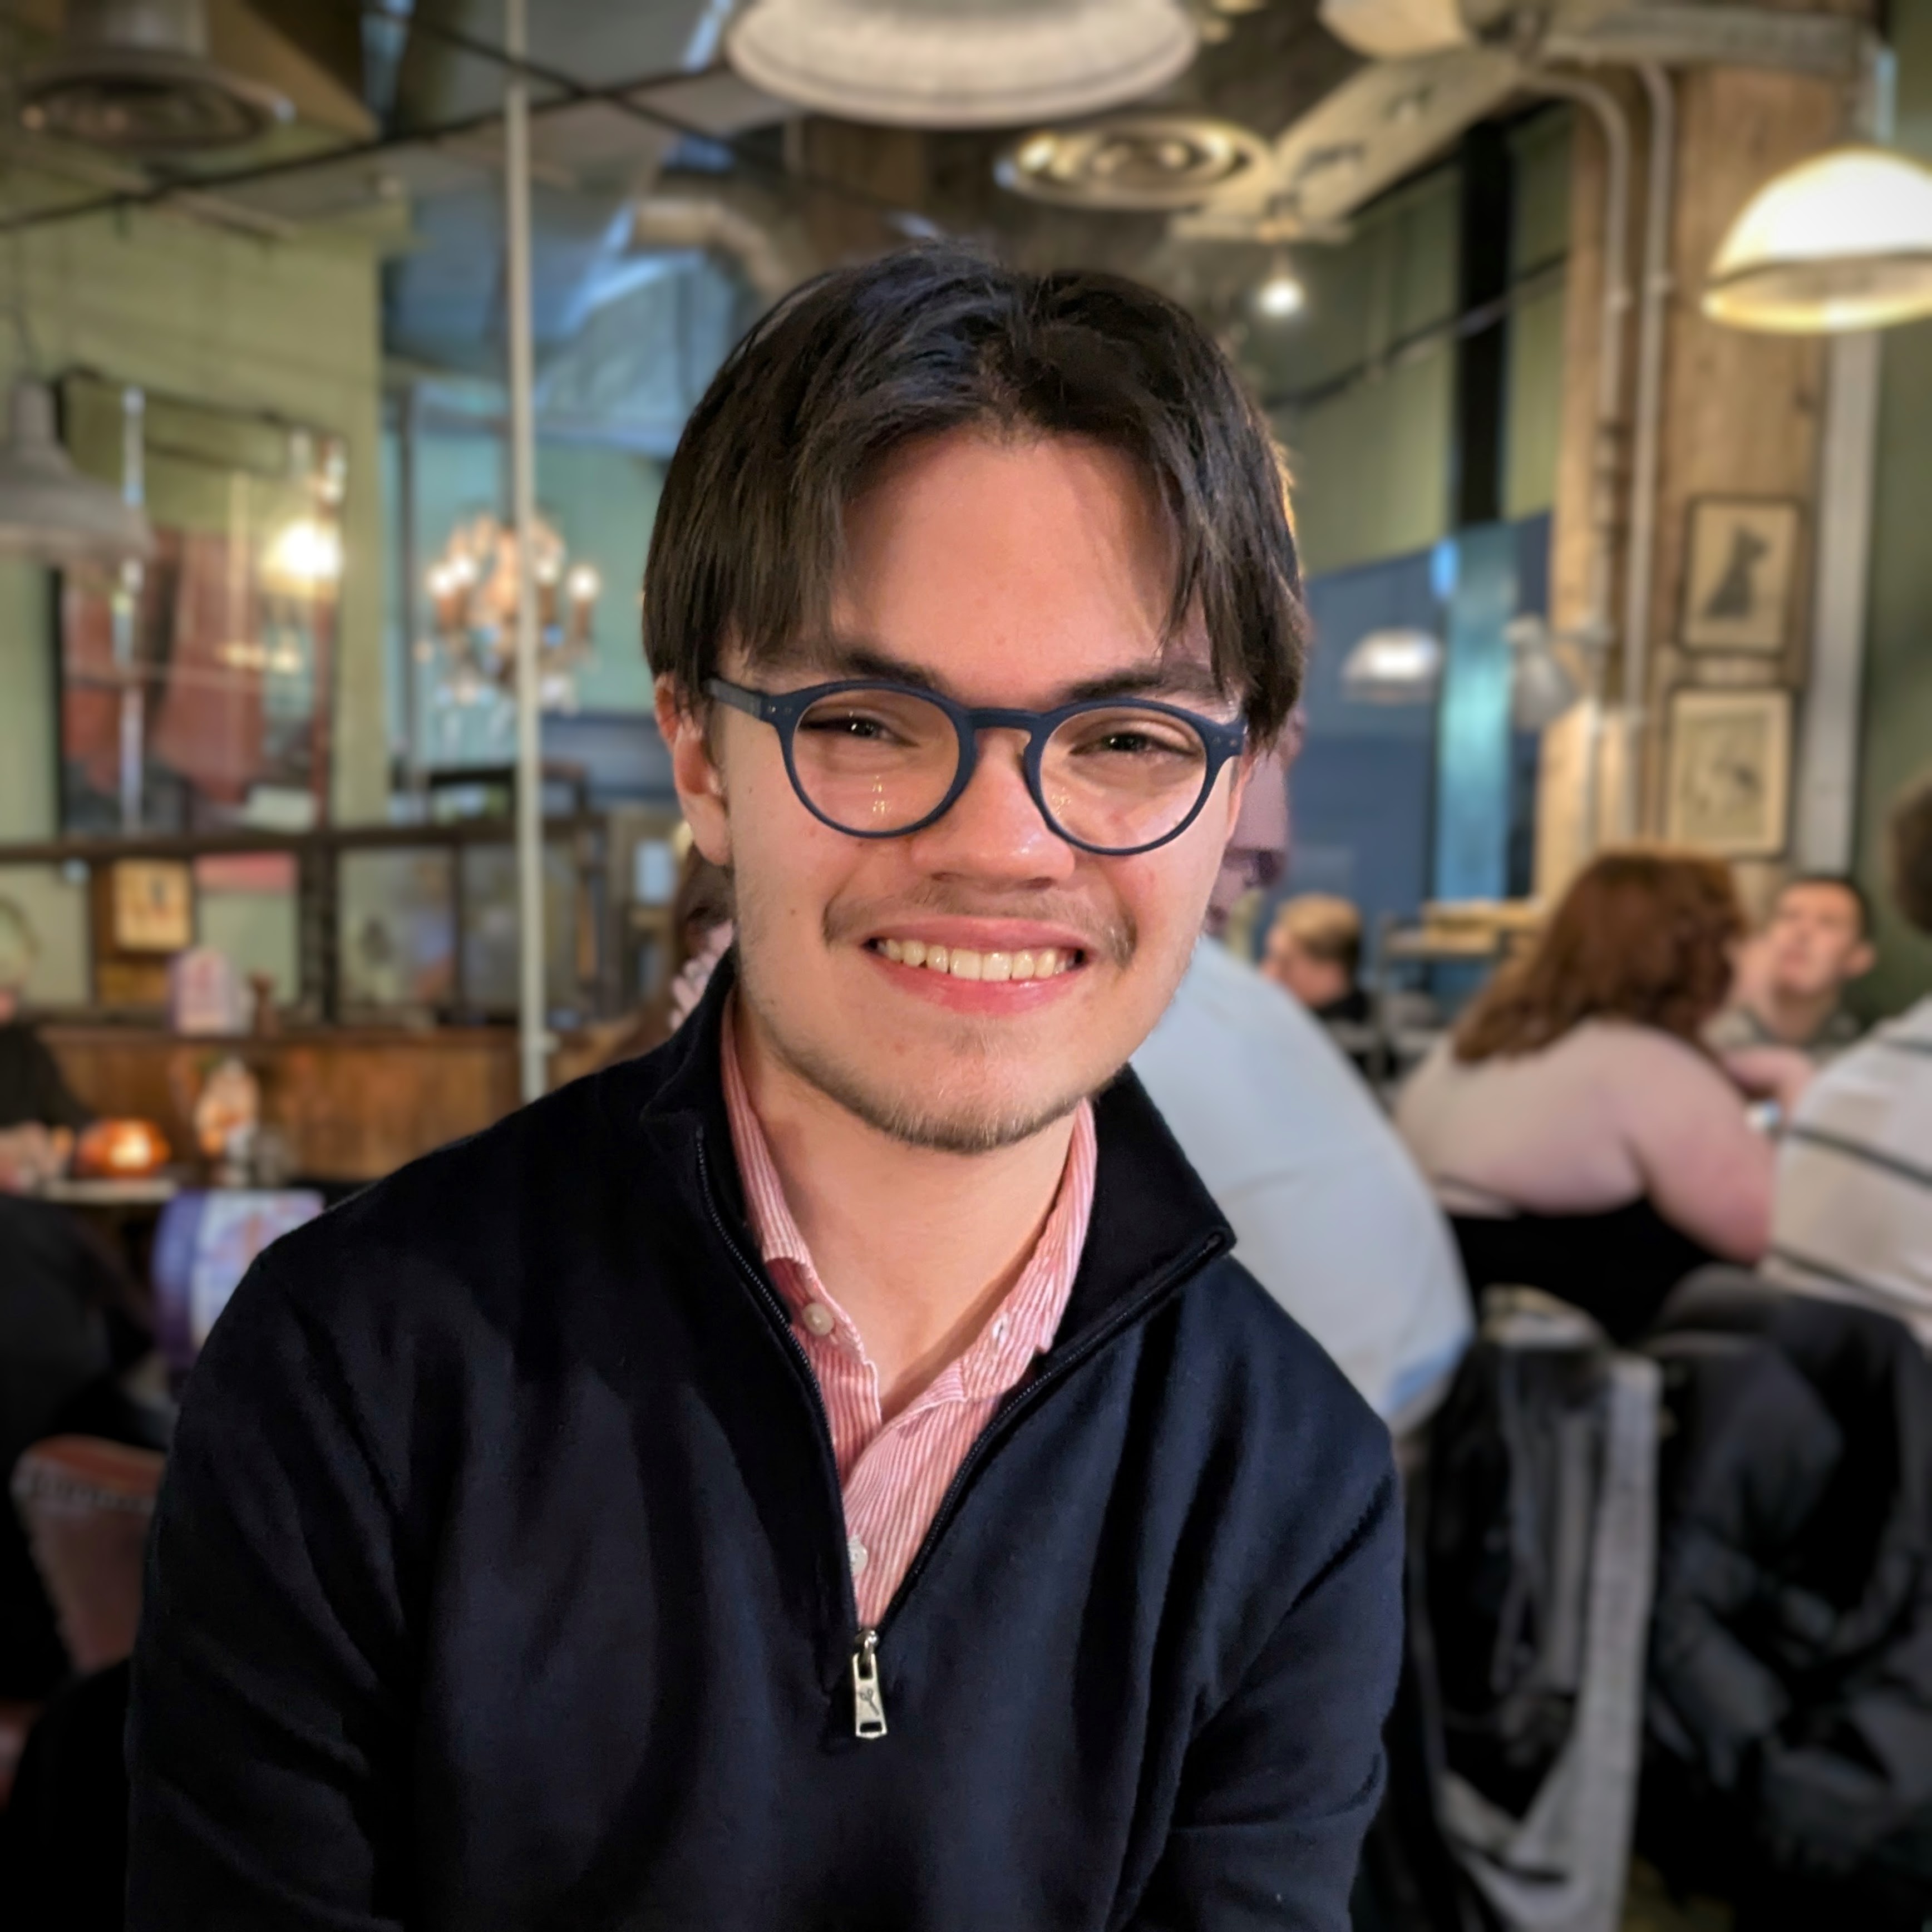
\includegraphics[width=1in,height=1.15in,clip,keepaspectratio]{figures/author_photo.jpg}}]{Dominic Bassett}
received the B.Sc. (Hons.) degree in Sound Engineering and Production with first-class honours from Birmingham City University, Birmingham, U.K., in 2026. His dissertation investigated spatial acuity and the resolution of directional information in spatial audio. He is a Graduate Acoustic Consultant with Cundall. His research interests include spatial audio signal processing, room-acoustic simulation, and perceptual modelling. He has also contributed to open-source acoustic modelling software, including binaural auralisation tools.
\end{IEEEbiography}

\vfill

\end{document}

